\documentclass[journal]{IEEEtran}

\usepackage[utf8]{inputenc}
\usepackage[spanish]{babel}
\usepackage{amsmath} % For equations
\usepackage{amsfonts} % For math fonts
\usepackage{amssymb} % For math symbols
\usepackage{graphicx} % For graphics
\usepackage{booktabs} % For better tables
\usepackage{url} % For hyperlinks
\usepackage{subfig} % Para subfiguras


\def\BibTeX{{\rm B\kern-.05em{\sc i\kern-.025em b}\kern-.08em
    T\kern-.1667em\lower.7ex\hbox{E}\kern-.125emX}}


\begin{document}

\title{Detección de Manchas Solares en Imágenes de Espectroheliógrafo H-Alpha Utilizando YOLOv8n}


\author{
    \IEEEauthorblockN{Ignacio Martínez Hernández} \\
    \IEEEauthorblockA{\textit{Doctorado Sistemas en Ingeniería} \\
        \textit{Machine Learning}\\
        \textit{Universidad de Talca}\\
        Curicó , Chile\\
        imartinez17@alumnos.utalca.cl}
}

\maketitle

\begin{abstract}
Este trabajo presenta una reimplementación y evaluación del problema de detección de manchas solares en imágenes de espectroheliógrafo H-Alpha, un desafío crucial
para la monitorización del clima espacial y el análisis de datos solares históricos. Basándose en un estudio previo que empleó la arquitectura YOLOv5 sobre el extenso dataset del Observatorio Geofísico y Astronómico de la Universidad de Coimbra (OGAUC) \cite{Santos2023}, este trabajo explora la aplicabilidad y el rendimiento de YOLOv8n, una versión más reciente y optimizada de la familia YOLO. Los resultados demuestran que, a pesar de ser la variante "nano" (más pequeña y eficiente), YOLOv8n alcanza métricas de rendimiento competitivas, destacando un mAP@.5 del 90.78\% y un mAP@.95 del 53.81\%, superando a los modelos YOLOv5 en esta última métrica más estricta. Adicionalmente, se demuestra la excelente capacidad de generalización del modelo al ser evaluado en un dataset externo sin re-entrenamiento, donde supera a un modelo de referencia en métricas clave. Estos hallazgos subrayan el potencial de YOLOv8n para aplicaciones robustas que requieren alta precisión de localización.
\end{abstract}

\begin{IEEEkeywords}
detección de manchas solares, redes neuronales convolucionales, YOLOv8, espectroheliógrafo, OGAUC
\end{IEEEkeywords}


\section{Contexto}
%La actividad solar ha sido objeto de una creciente investigación en las últimas décadas debido a su significativa influencia en la vida en la Tierra. Fenómenos como las eyecciones de masa coronal (CME), las partículas energéticas solares y las erupciones pueden interrumpir las comunicaciones por satélite, las herramientas de navegación e incluso las redes eléctricas y otras infraestructuras críticas para nuestra sociedad tecnológica. La predicción de estos eventos es posible mediante la monitorización del Sol y el análisis de imágenes obtenidas en diferentes espectros, lo que permite identificar fenómenos como filamentos, poros y manchas solares. El Observatorio Geofísico y Astronómico de la Universidad de Coimbra (OGAUC) ha monitorizado la actividad solar desde 1926, acumulando uno de los datasets más antiguos y completos de imágenes solares a nivel mundial. Dada la vasta cantidad de imágenes disponibles, los métodos automáticos para detectar y rastrear manchas solares representan una mejora fundamental en el campo de la monitorización del clima espacial. Trabajos previos han explorado la detección de manchas solares utilizando enfoques tradicionales y, más recientemente, redes neuronales convolucionales (CNNs). La arquitectura YOLO (You Only Look Once) se ha consolidado como una de las CNNs más populares para la detección de objetos debido a su eficiencia y velocidad. El estudio original, en el que se basa esta reimplementación, aplicó YOLOv5 con éxito para la detección de manchas solares en el dataset del OGAUC, alcanzando un mAP@.5 superior al 90\% \cite{Santos2023}. El presente trabajo tiene como objetivo reevaluar la detección de manchas solares en el mismo dataset del OGAUC, pero empleando la arquitectura YOLOv8n (nano). Este estudio busca comparar el rendimiento de YOLOv8n con las variantes de YOLOv5 reportadas previamente, proporcionando una visión actualizada sobre la eficiencia de modelos de detección de objetos más recientes y ligeros en este dominio.
La actividad solar ha sido objeto de una creciente investigación en las últimas décadas debido a su significativa influencia en la vida en la Tierra. Para predecir eventos solares peligrosos, es crucial monitorizar el Sol analizando imágenes. Una técnica clave para esto es el uso del \textbf{espectroheliógrafo H-Alpha}. En términos sencillos, este instrumento es como una cámara con un filtro muy específico que solo deja pasar un tipo de luz roja emitida por el hidrógeno en la atmósfera del Sol. Al hacer esto, revela una capa solar normalmente invisible (la cromosfera), permitiendo ver claramente las zonas de alta actividad magnética donde se originan las manchas solares. Fenómenos como las eyecciones de masa coronal (CME) y las erupciones, que pueden interrumpir tecnologías críticas en la Tierra, están directamente relacionados con esta actividad. El Observatorio Geofísico y Astronómico de la Universidad de Coimbra (OGAUC) ha utilizado esta técnica desde 1926, creando un valioso archivo histórico. Dada la enorme cantidad de imágenes, los métodos automáticos para detectar manchas solares son fundamentales. La arquitectura YOLO (You Only Look Once) se ha destacado por su eficiencia en esta tarea. El estudio original \cite{Santos2023} usó YOLOv5 con éxito en el dataset del OGAUC. Este trabajo busca reevaluar el problema empleando YOLOv8n, una versión más moderna y ligera, para comparar su rendimiento y eficiencia.


\section{Planteamiento del Problema}
La detección precisa y automática de manchas solares es un desafío fundamental en la heliofísica. Las manchas solares, regiones más frías y oscuras en la superficie solar causadas por fuertes campos magnéticos, son indicadores clave de la actividad solar y precursores de fenómenos como las erupciones solares que impactan el clima espacial. Históricamente, la detección y clasificación de manchas solares se ha realizado mediante observación manual, un proceso laborioso, propenso a errores y poco escalable para el análisis de grandes volúmenes de datos históricos. Además, las imágenes de espectroheliógrafos terrestres, como las del OGAUC, presentan desafíos inherentes como la variabilidad en la calidad debido a las condiciones atmosféricas y la presencia de anotaciones directas en la imagen. La necesidad de métodos automatizados y robustos que puedan procesar eficientemente estos archivos históricos es imperativa para comprender la evolución de los ciclos solares y su impacto a largo plazo en la Tierra. El problema se centra en desarrollar un sistema capaz de identificar con alta precisión las manchas solares dentro de estas imágenes complejas, superando las limitaciones de los métodos manuales y las dificultades intrínsecas de los datos.
\section{Propuesta de Solución}
Para abordar el problema de la detección automática de manchas solares, se propone el uso de redes neuronales convolucionales (CNNs) para la detección de objetos. Las CNNs han demostrado ser excepcionalmente versátiles y eficientes para el análisis de imágenes, destacándose en tareas de detección y clasificación. El estudio original eligió la arquitectura YOLOv5 (You Only Look Once, versión 5) debido a su alto rendimiento y capacidad para procesar grandes volúmenes de datos en tiempos razonables \cite{Santos2023}. En esta reimplementación, esta solución consiste en sustituir el modelo YOLOv5 por \textbf{YOLOv8n (nano)}. YOLOv8n es una versión más reciente de la familia YOLO, desarrollada por Ultralytics, que se caracteriza por ser una arquitectura más ligera y optimizada, diseñada para ofrecer una inferencia más rápida con un menor consumo de recursos computacionales. La elección de la variante "nano" se justifica por su equilibrio entre eficiencia y rendimiento, lo que la hace particularmente atractiva para aplicaciones donde la velocidad de procesamiento es crítica o los recursos de hardware son limitados. Esta adaptación busca confirmar si un modelo de menor complejidad puede mantener un rendimiento competitivo en comparación con sus predecesores, en el contexto específico de la detección de manchas solares en imágenes históricas de espectroheliógrafo.
\section{Metodología}
La metodología seguida en esta reimplementación se alinea con la del estudio original \cite{Santos2023}, con la principal diferencia en el modelo de detección de objetos empleado.
\subsection{Adquisición de Datos}
El dataset empleado en esta reimplementación es el conjunto de datos \textbf{final procesado y compartido} por los autores del artículo original \cite{Santos2023}. Este dataset\footnote{\url{https://www.kaggle.com/datasets/aaiisec/ogauc-solar-images-marked-for-yolo-cnn-cycle-24/}} se generó a partir de una colección inicial de 2000 imágenes de continuo H-alpha, con una resolución de 1200x1000 píxeles, obtenidas del espectroheliógrafo terrestre del Observatorio Geofísico y Astronómico de la Universidad de Coimbra (OGAUC) entre el 15 de febrero de 2012 y el 26 de abril de 2019 (Ciclo Solar 24). Es importante señalar que, al ser imágenes terrestres, estas pueden presentar desafíos como ruido, variaciones en la calidad debido a las condiciones atmosféricas (seeing, transparencia atmosférica) y posibles artefactos instrumentales, lo que añade complejidad a la tarea de detección. Los autores del paper original aplicaron un riguroso proceso de pre-procesamiento y aumento de datos a esta colección inicial para crear el conjunto de datos específico utilizado en sus experimentos finales \cite{Santos2023}. Este dataset resultante, el cual se empleó directamente en esta reimplementación, está compuesto por 3247 imágenes para el entrenamiento y 600 imágenes para la validación, sumando un total de 3847 imágenes. Este conjunto ya incorpora las transformaciones y anotaciones necesarias para el modelado.
\subsection{Pre-procesamiento}


El dataset empleado en esta reimplementación ya incorpora los pasos de pre-procesamiento esenciales realizados por los autores del estudio original \cite{Santos2023}. Específicamente, las imágenes fueron previamente recortadas para eliminar anotaciones y las áreas negras periféricas alrededor del disco solar, enfocando así la región de interés para la detección de manchas solares. Además del recorte, los autores originales aplicaron técnicas de \textbf{aumento de datos} para incrementar la robustez y el tamaño del dataset \cite{Santos2023}. Estas técnicas incluyeron:
\begin{itemize}
    \item Volteos horizontales y verticales.
    \item Una transformación de cizallamiento (shear transform).
\end{itemize}

Dado que el conjunto de datos ya estaba aumentado, en esta reimplementación se desactivaron explícitamente las opciones de aumento de datos adicionales durante el entrenamiento de YOLOv8n. Esto se hizo para evitar la sobre-aplicación de transformaciones y asegurar una comparación más directa y justa, evaluando el rendimiento del modelo sobre el dataset pre-procesado tal como fue proporcionado por los autores originales \cite{Santos2023}.
\subsection{Modelado}
El proceso de modelado implicó el entrenamiento de la arquitectura YOLOv8n para la tarea de detección de manchas solares. Dado que el objetivo es únicamente identificar la presencia de manchas solares, el problema se aborda como una tarea de detección de una sola clase (binaria): "sunspot". YOLOv8n es la versión más compacta de la serie YOLOv8 desarrollada por Ultralytics, que incorpora mejoras en la arquitectura y el proceso de entrenamiento respecto a versiones anteriores de YOLO. Para esta reimplementación, se utilizó el modelo pre-entrenado \texttt{yolov8n.pt} y se ajustó a medida (\textit{fine-tuned}) utilizando el dataset preparado. La configuración de entrenamiento específica fue la siguiente:
\begin{itemize}
    \item \textbf{Épocas:} 20
    \item \textbf{Tamaño de imagen de entrada (\texttt{imgsz}):} 640x640 píxeles
    \item \textbf{Tamaño de lote (\texttt{batch}):} 16
    \item \textbf{Aumento de datos:} Desactivado
\end{itemize}

Siguiendo las mismas características que la implementación original \cite{Santos2023}, salvo en las épocas de entrenamiento. El modelo original fue entrenado durante 300 épocas, una cantidad significativamente mayor que las 20 épocas utilizadas en esta reimplementación \cite{Santos2023}. Esta diferencia hace que los resultados competitivos obtenidos sean aún más notables, destacando la eficiencia de la arquitectura YOLOv8n.
\subsection{Validación}
Para la evaluación del rendimiento del modelo, se utilizaron las siguientes métricas clave en detección de objetos: Precisión (P), Recall (R) y \textit{mean Average Precision} (mAP).
\begin{itemize}
    \item \textbf{Precisión (Precision - P):} Mide la proporción de detecciones correctas (verdaderos positivos) entre todas las detecciones realizadas por el modelo. Indica qué tan fiable es el modelo cuando detecta un objeto. \[ P = \frac{TP}{TP+FP} \]
    \item \textbf{Recall (Exhaustividad - R):} Mide la proporción de verdaderos positivos que fueron detectados correctamente por el modelo, entre todos los objetos reales presentes en las imágenes. Indica la capacidad del modelo para encontrar todas las instancias relevantes. \[ R = \frac{TP}{TP+FN} \]
    \item \textbf{True Positive (TP):} El modelo detectó correctamente una mancha solar real.
    \item \textbf{False Positive (FP):} El modelo detectó una mancha solar donde no había ninguna (detección incorrecta).
    \item \textbf{False Negative (FN):} El modelo no detectó una mancha solar real (error de omisión).
    \item \textbf{Mean Average Precision (mAP):} Es una métrica comúnmente utilizada en la detección de objetos que promedia los valores de Precision Media (AP) para todas las clases y para múltiples umbrales de \textit{Intersection over Union} (IoU). Un umbral de IoU de 0.5, por ejemplo (mAP@.5), significa que una detección se considera un verdadero positivo si su \textit{bounding box} se solapa al menos un 50\% con el \textit{bounding box} real. El mAP@.95 es una métrica más estricta, que requiere un solapamiento del 95\%. Estas métricas proporcionan una evaluación integral del rendimiento del modelo en términos de precisión de localización y clasificación.
\end{itemize}

\section{Resultados}
La siguiente tabla compara el rendimiento de los modelos YOLOv5 (s, m, l) reportados en el estudio original \cite{Santos2023} con los resultados obtenidos utilizando YOLOv8n, sobre el mismo dataset.
\begin{table}[htbp]
\centering
\caption{Comparación de Métricas de Rendimiento}
\label{tab:results_comparison}
\begin{tabular}{@{}lllll@{}}
\toprule
\textbf{Modelo} & \textbf{Precisión} & \textbf{Recall} & \textbf{mAP@.5} & \textbf{mAP@.95} \\
\midrule
YOLOv5s & 88.85\% & 82.31\% & 90.43\% & 49.14\% \\
YOLOv5m & 88.90\% & 82.95\% & 91.14\% & 51.44\% \\
YOLOv5l & 90.00\% & 82.38\% & 91.53\% & 52.71\% \\
\textbf{YOLOv8n} & \textbf{86.80\%} & \textbf{84.35\%} & \textbf{90.78\%} & \textbf{53.81\%} \\
\bottomrule
\label{tab:comparison_results}
\end{tabular}
\end{table}

Para ofrecer un análisis más detallado del rendimiento de YOLOv8n en el conjunto de validación, la Tabla \ref{tab:confusion_matrix} presenta la matriz de confusión. Esta matriz desglosa las predicciones del modelo, mostrando el número de Verdaderos Positivos (manchas solares correctamente identificadas), Falsos Negativos (manchas solares no detectadas) y Falsos Positivos (detecciones incorrectas en el fondo).
\begin{table}[htbp]
\centering
\caption{Matriz de Confusión para YOLOv8n}
\label{tab:confusion_matrix}
\begin{tabular}{@{}l|cc@{}}
\toprule
\textbf{} & \multicolumn{2}{c}{\textbf{Clase Predicha}} \\
\textbf{Clase Real} & \textbf{Sunspot} & \textbf{Background (No detectado)} \\
\midrule
\textbf{Sunspot} & 1424 (TP) & 315 (FN) \\
\textbf{Background} & 154 (FP) & - \\
\bottomrule
\end{tabular}
\end{table}

La matriz muestra que el modelo identificó correctamente 1424 instancias de manchas solares, mientras que omitió 315. Además, generó 154 detecciones falsas. Estos valores son la base para el cálculo de las métricas de Precisión y Recall presentadas en la Tabla \ref{tab:results_comparison}.

\begin{figure*}[t]
    \centering
    \subfloat[Imagen Original]{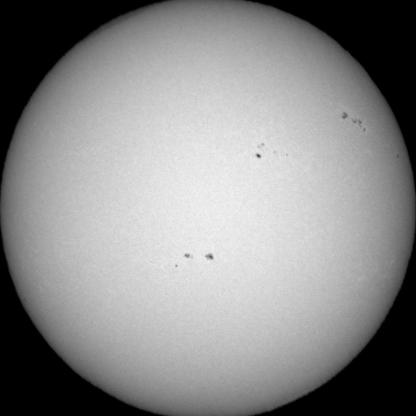
\includegraphics[width=0.30\textwidth]{./image_original.jpg}\label{fig:original}}
    \hfil
    \subfloat[Etiquetas Reales (Ground Truth)]{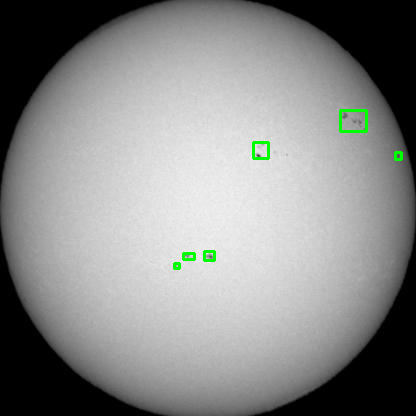
\includegraphics[width=0.30\textwidth]{./image_label.png}\label{fig:labels}}
    \hfil
    \subfloat[Predicciones del Modelo YOLOv8n]{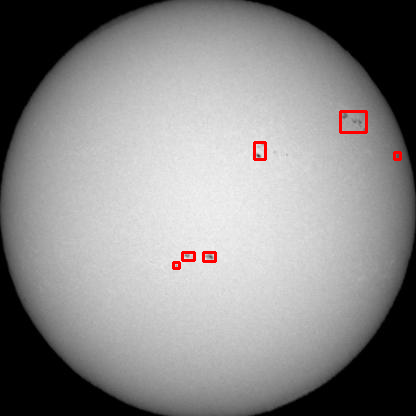
\includegraphics[width=0.30\textwidth]{./image_predicted.png}\label{fig:predicted}}
    \caption{Comparación visual de un ejemplo de detección. (a) Imagen de entrada del espectroheliógrafo. (b) Las cajas delimitadoras reales que marcan las manchas solares. (c) Las cajas delimitadoras predichas por el modelo YOLOv8n, demostrando una alta correspondencia con las etiquetas reales.}
    \label{fig:visual_comparison}
\end{figure*}


\subsection{Evaluación de Generalización en un Dataset Externo}

Para evaluar la capacidad de generalización del modelo entrenado, se realizó una evaluación adicional utilizando un segundo dataset completamente independiente\footnote{\url{https://universe.roboflow.com/internship-projects/sunspot-detection-using-yolov5}}, que abarca diferentes periodos de observación solar. Es crucial destacar que el modelo YOLOv8n \textbf{no fue re-entrenado} en este nuevo conjunto de datos; se utilizó directamente el modelo entrenado con los datos del OGAUC. Este nuevo dataset cuenta con sus propias divisiones de validación y prueba, y se ha publicado previamente un modelo de referencia con métricas de rendimiento conocidas. La Tabla \ref{tab:generalization_results} presenta los resultados obtenidos por nuestro modelo en este dataset externo, comparándolos con el modelo de referencia publicado para dicho conjunto de datos.
\begin{table}[htbp]
\centering
\caption{Rendimiento del Modelo YOLOv8n en un Dataset Externo No Visto}
\label{tab:generalization_results}
\begin{tabular}{@{}lcccc@{}}
\toprule
\textbf{Modelo / Conjunto} & \textbf{Precisión} & \textbf{Recall} & \textbf{mAP@.5} & \textbf{mAP@.95} \\
\midrule
\textbf{Nuestro} - Val & 89.77\% & 87.53\% & 93.81\% & 56.65\% \\
\textbf{Nuestro} - Test & \textbf{90.60\%} & \textbf{88.35\%} & \textbf{94.41\%} & \textbf{57.39\%} \\
\midrule
Modelo de Referencia & 90.50\% & 91.30\% & 93.60\% & - \\
\bottomrule
\end{tabular}
\end{table}

Los resultados en el conjunto de prueba (\textit{test set}) son particularmente notables. Nuestro modelo YOLOv8n, sin entrenamiento previo en estos datos, alcanza una Precisión (90.60\%) y un mAP@.5 (94.41\%) que superan al modelo de referencia, el cual fue específicamente entrenado para este dataset. Aunque el Recall es ligeramente inferior (88.35\% vs 91.30\%), el rendimiento general demuestra una excelente capacidad de generalización. Adicionalmente, se obtiene un mAP@.95 de 57.39\%, un valor robusto que, si bien no tiene contraparte en el modelo de referencia, confirma la alta calidad en la localización de las detecciones. Para un análisis más detallado de este rendimiento, la Tabla \ref{tab:confusion_matrix_external} presenta la matriz de confusión para el conjunto de prueba del dataset externo.
\begin{table}[htbp]
\centering
\caption{Matriz de Confusión para YOLOv8n en el Test Set del Dataset Externo}
\label{tab:confusion_matrix_external}
\begin{tabular}{@{}l|cc@{}}
\toprule
\textbf{} & \multicolumn{2}{c}{\textbf{Clase Predicha}} \\
\textbf{Clase Real} & \textbf{Sunspot} & \textbf{Background (No detectado)} \\
\midrule
\textbf{Sunspot} & 956 (TP) & 161 (FN) \\
\textbf{Background} & 70 (FP) & - \\
\bottomrule
\end{tabular}
\end{table}

La matriz de confusión del conjunto de prueba externo cuantifica la robustez del modelo: identificó correctamente 956 manchas solares (TP) y generó únicamente 70 falsos positivos (FP), lo que se alinea con la alta Precisión reportada. Al mismo tiempo, omitió 161 manchas solares (FN), lo que es consistente con el valor de Recall. Este desglose confirma que el modelo, incluso en datos no vistos, mantiene un excelente equilibrio entre detectar correctamente las manchas existentes y evitar detecciones erróneas.
\section{Discusión}

El análisis de resultados revela un perfil de rendimiento para YOLOv8n que es tanto competitivo como estratégicamente ventajoso. Frente a las variantes de YOLOv5 (Tabla \ref{tab:results_comparison}), YOLOv8n demuestra una superioridad en la métrica más exigente, mAP@.95 (53.81\% vs. 52.71\% de YOLOv5l), lo que indica una localización de objetos más precisa. Si bien su Precisión (86.80\%) y mAP@.5 (90.78\%) son comparables a las de los modelos más grandes de YOLOv5, su principal ventaja radica en el Recall (84.35\%), el más alto de todos los modelos comparados. Este atributo es crucial en aplicaciones de monitorización, donde minimizar los falsos negativos (manchas no detectadas) es prioritario.

\textbf{El hallazgo más significativo de este estudio proviene de la evaluación de generalización (Tabla \ref{tab:generalization_results}).} Al probar el modelo entrenado con datos del OGAUC en un dataset externo completamente nuevo y sin re-entrenamiento, no solo mantuvo un alto rendimiento, sino que superó al modelo de referencia (entrenado específicamente para esos datos) en Precisión (90.60\% vs. 90.50\%) y mAP@.5 (94.41\% vs. 93.60\%). Este hecho subraya de manera contundente que el modelo no se ha sobreajustado al dataset original, sino que ha aprendido características fundamentales y transferibles de las manchas solares, validando su robustez para ser usado en datos de diversas fuentes.

El análisis de las matrices de confusión (Tablas \ref{tab:confusion_matrix} y \ref{tab:confusion_matrix_external}) refuerza estas observaciones. En ambos datasets, el modelo muestra una tendencia a favorecer un alto número de Verdaderos Positivos a costa de algunos Falsos Positivos, lo que es consistente con su alto Recall. En conjunto, YOLOv8n se perfila como un modelo excepcionalmente eficiente: es capaz de encontrar más manchas solares (alto Recall), localizarlas con una precisión espacial muy alta (alto mAP@.95) y generalizar su conocimiento a datos no vistos, todo ello con una arquitectura ligera y en un número reducido de épocas de entrenamiento.

Para explorar los límites de la generalización, se realizó un experimento adicional sobre el segundo dataset, el cual es significativamente más grande que el conjunto de OGAUC (4046 imágenes de entrenamiento vs. 3247). De manera sorprendente, el entrenamiento por transferencia no solo no mejoró el rendimiento, sino que lo degradó. El punto óptimo se alcanzó en la primera época (mAP@.5 de 91.56\%), un valor inferior al 94.41\% obtenido sin re-entrenamiento, y las métricas continuaron decayendo en épocas posteriores. Este hallazgo es particularmente revelador: sugiere que el modelo entrenado en el dataset OGAUC, aunque más pequeño, aprendió un conjunto de características más robustas y generalizables. El intento de especialización en el dataset más grande, pero potencialmente más heterogéneo o con mayor ruido, resultó contraproducente, corrompiendo el conocimiento de alta calidad ya adquirido.

\section{Conclusión}

Este trabajo ha demostrado con éxito la eficacia del modelo YOLOv8n para la detección de manchas solares en imágenes históricas de espectroheliógrafo H-Alpha del dataset OGAUC. La reimplementación no solo validó la viabilidad de utilizar arquitecturas modernas y ligeras para esta tarea, sino que también reveló que YOLOv8n ofrece un rendimiento altamente competitivo frente a los modelos YOLOv5 de referencia. En particular, destaca por alcanzar los valores más altos tanto en Recall (84.35\%) como en mAP@.95 (53.81\%), indicando que es capaz de encontrar más manchas solares y localizarlas con mayor precisión espacial.

La contribución más significativa de este estudio es la demostración de la \textbf{excelente capacidad de generalización} del modelo. Al ser evaluado en un dataset externo completamente nuevo, sin ningún tipo de re-entrenamiento, el modelo YOLOv8n no solo mantuvo su robustez, sino que superó en métricas clave como Precisión (90.60\%) y mAP@.5 (94.41\%) a un modelo de referencia específicamente entrenado para dichos datos. Este resultado confirma que el modelo ha aprendido características fundamentales y transferibles de las manchas solares, posicionándolo como una herramienta fiable y robusta para el análisis de datos solares de diversas fuentes.

En definitiva, YOLOv8n se consolida como una solución eficiente y potente, que ofrece un notable equilibrio entre rendimiento y ligereza computacional, ideal para la monitorización del clima espacial y el análisis de grandes archivos históricos.

Como trabajo futuro, se perfila una hoja de ruta ambiciosa para evolucionar este proyecto desde un detector de objetos a un sistema de análisis solar integral e interpretable. El primer paso crucial será validar y extender el modelo actual utilizando imágenes satelitales de alta resolución del Solar Dynamics Observatory (SDO), para asegurar su robustez y aplicabilidad en datos de calidad profesional. A continuación, se planea ampliar la capacidad del sistema más allá de la detección, implementando una etapa de clasificación de manchas solares (p. ej., según el esquema de McIntosh). La línea de investigación más innovadora consistirá en integrar técnicas de IA Explicable (XAI) para visualizar qué características de la imagen (umbra, penumbra, complejidad) fundamentan las decisiones del modelo. Finalmente, se propone utilizar un Modelo de Lenguaje Grande (LLM) que reciba como entrada la detección, la clasificación y el mapa de explicabilidad de XAI, con el objetivo de generar una descripción en lenguaje natural que justifique el hallazgo como lo haría un astrónomo experto. Este enfoque no solo busca mejorar la fiabilidad de los resultados, sino también construir un sistema transparente y confiable para la comunidad científica y los observatorios.



\begin{thebibliography}{00}
    \bibitem{Santos2023}
    J.~Santos, N.~Peixinho, T.~Barata, C.~Pereira, A.~P.~Coimbra, M.~M.~Crisóstomo, and M.~Mendes, ``Sunspot Detection Using YOLOv5 in Spectroheliograph H-Alpha Images,'' \emph{Applied Sciences}, vol.~13, no.~10, Art.
no. 5833, 2023. [Online]. Available: \url{https://www.mdpi.com/2076-3417/13/10/5833}. doi:10.3390/app13105833

    \bibitem{Kaggle2022}
    AI \& Intelligent Systems Lab, ``OGAUC Solar Images Marked for YOLO CNN (Cycle 24),'' \textit{Kaggle}, 2022. [Online]. Available: \url{https://www.kaggle.com/datasets/aaiisec/ogauc-solar-images-marked-for-yolo-cnn-cycle-24}

    \bibitem{Roboflow2022}
    Roboflow Internship Projects, ``Sunspot Detection using YOLOv5,'' \textit{Roboflow Universe}, 2022. [Online]. Available: \url{https://universe.roboflow.com/internship-projects/sunspot-detection-using-yolov5}

\end{thebibliography}

\end{document}